% !TEX root = ../main.tex
% SECTION 8: SCHRAUBEN
% Inhalt: Liv Erne, Silvio Seiz — Form: ZSF-Template-Rework
% ============================================================

\StartChapter[ch:schrauben]{Schrauben}
\ZSFindex{Schraube}

\begin{runintext}
Mit Schraubenmutter, Innengewinde, Schraubenkopf, Schraubenschaft und Aussengewinde.
\end{runintext}

\begin{formulabox}
\ZSFkeyword*{Eindrehwinkel und Weg}:~$\ZSFscrewAlpha = \dfrac{\ZSFscrewS}{\ZSFscrewP}\cdot 360° \qquad \ZSFscrewS = \dfrac{\ZSFscrewAlpha}{360°}\cdot \ZSFscrewP$
\formulanote{$\ZSFscrewAlpha =$ Eindrehwinkel, $\ZSFscrewS =$ Weg, $\ZSFscrewP =$ Steigung}
\end{formulabox}

\begin{tablebox}[Schraubenköpfe]
\renewcommand{\arraystretch}{1.3}
\begin{ZSFtable}[\ZSFfontTableDense]{Z{0.75} Z{1.25} Z{1.125} Z{0.75} Z{1.125}}
\ZSFheaderRow \ZSFhead{Kopf} & \ZSFhead{Name} & \ZSFhead{Anzieh\-moment} & \ZSFhead{Preis} & \ZSFhead{Montage} \\

\includegraphics[width=0.65\hsize,keepaspectratio]{graphics/v10_slotted_screw_drive.png} & Längsschlitz & niedrig & günstig & schlechte Zentrierung \\

\includegraphics[width=0.65\hsize,keepaspectratio]{graphics/v10_schraubenantrieb_kreuzschlitz.png} & Kreuzschlitz & niedrig & günstig & gute Zentrierung \\

\includegraphics[width=0.65\hsize,keepaspectratio]{graphics/v10_schraubenkopf_aussensechskant.png} & Aussensechskant & hoch & günstig & grosser Platzbedarf \\

\includegraphics[width=0.65\hsize,keepaspectratio]{graphics/v10_schraubenantrieb_innensechskant.png} & Innensechskant (Imbus) & mittel & günstig & wenig Platzbedarf \\

\includegraphics[width=0.65\hsize,keepaspectratio]{graphics/v10_schraubenkopf_aussenvielzahn.png} & Aussenvielzahn & sehr hoch & teuer & grosser Platzbedarf \\

\includegraphics[width=0.65\hsize,keepaspectratio]{graphics/v10_schraubenantrieb_innenvielzahn_torx.png} & Innenvielzahn (Torx) & hoch & teuer & wenig Platzbedarf
\end{ZSFtable}
\end{tablebox}
\ZSFindex[schraubenkopfe]{Schraubenköpfe}

\SubsectionBar[sec:gewinde]{Gewinde}
\ZSFindex{Gewinde}

\begin{runintext}
Wandelt Rotation in Translation. Links- und Rechtsgewinde (Standard).
\end{runintext}

\begin{valuegrid}{1}[Gewindearten]
Metrisch & $\ZSFscrewBeta = 60^\circ$ \\
Whitworth & $\ZSFscrewBeta = 55^\circ$ \\
Trapez & $\ZSFscrewBeta = 30^\circ$ \\
Sägen & $\ZSFscrewBeta = 30^\circ$ resp. $3^\circ$
\end{valuegrid}

\begin{valuegridtwo}[Metrisches Gewinde (Beispiele)]
Regelgewinde & M10 & $\ZSFscrewD = 10\,\text{mm}, \ZSFscrewP = 1.5\,\text{mm}$ \\
Feingewinde & $M10\times 1.25$ & $\ZSFscrewD = 10\,\text{mm}, \ZSFscrewP = 1.25\,\text{mm}$
\end{valuegridtwo}
\ZSFindex{Feingewinde}
\ZSFindex{Gewinde, metrisches}

\begin{formulabox}[Gewindeprofil (ISO)]
\[ \ZSFscrewH = \dfrac{\sqrt{3}}{2}\cdot \ZSFscrewP \qquad \ZSFscrewHThree = \ZSFscrewH - \dfrac{\ZSFscrewH}{6}- \dfrac{\ZSFscrewH}{8} \]
\formulanote{$\ZSFscrewH$:~Profilhöhe \ $\cdot$ \ $\ZSFscrewHThree$:~Gewindetiefe \ $\cdot$ \ $\ZSFscrewP$:~Steigung}
\end{formulabox}

\begin{figbox}[Gewindegeometrie]
\begin{minipage}[c]{0.54\linewidth}\centering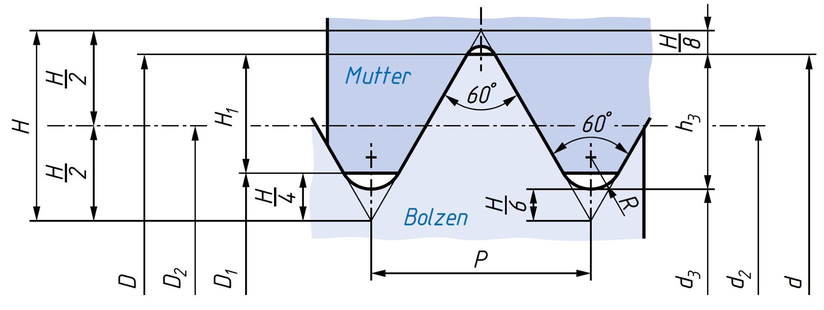
\includegraphics[width=\linewidth,keepaspectratio]{graphics/v10_schrauben_metrisches_iso_gewinde.png}\end{minipage}\hfill\begin{minipage}[c]{0.42\linewidth}\centering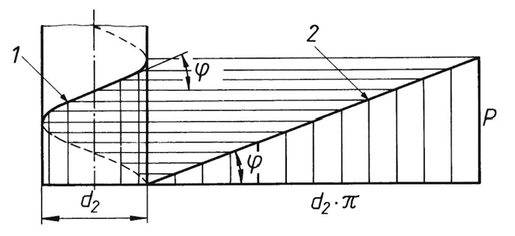
\includegraphics[width=\linewidth,keepaspectratio]{graphics/v10_schrauben_gewinde_kennwerte.png}\end{minipage}
\end{figbox}

\ZSFfig[0.85]{graphics/v10_schraubenquerschnitte.png}{}{}

\begin{formulabox}[Steigungswinkel \& Querschnitte]
\[ \tan \ZSFscrewPhi = \dfrac{\ZSFscrewP}{\ZSFscrewDTwo \cdot \pi} \qquad \ZSFscrewDs = \dfrac{1}{2} \cdot (\ZSFscrewDTwo + \ZSFscrewDThree) \]
\formulanote{$\ZSFscrewPhi$:~Steigungswinkel \ $\cdot$ \ $\ZSFscrewDTwo$:~Flankend. \ $\cdot$ \ $\ZSFscrewDThree$:~Kernd. \ $\cdot$ \ $\ZSFscrewDs$:~Spannungsd. \ $\cdot$ \ $\ZSFscrewA = \ZSFscrewAN$:~Nennquerschn. \ $\cdot$ \ $\ZSFscrewAk = \ZSFscrewAThree$:~Kernquerschn.}
\end{formulabox}

\SubsectionBar[sec:festigkeitsklassen]{Festigkeitsklassen}
\ZSFindex{Festigkeitsklasse}

\begin{figbox}
\centering
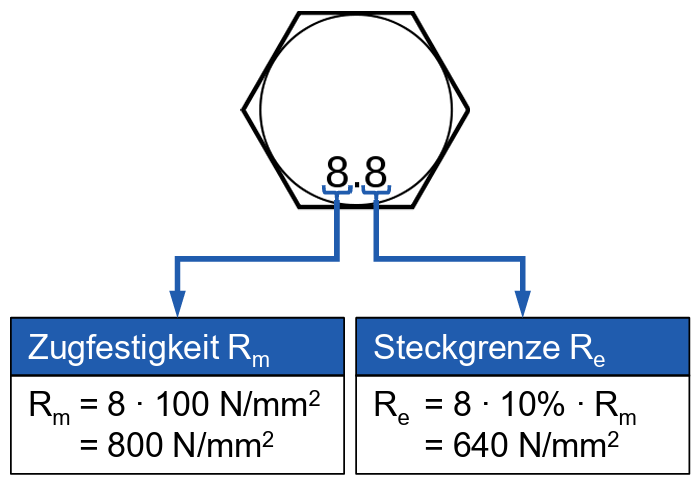
\includegraphics[width=0.38\linewidth,keepaspectratio]{graphics/v10_schraube_festigkeitsklasse_beispiel_8_8.png}%
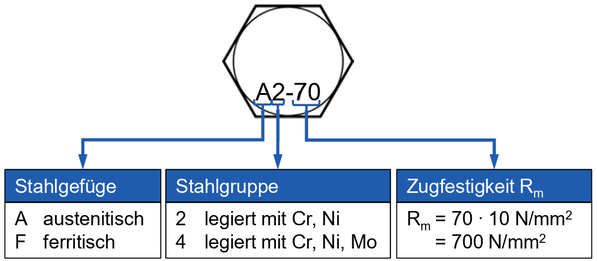
\includegraphics[width=0.58\linewidth,keepaspectratio]{graphics/v10_schraube_festigkeitsklassen_tabelle.png}
\end{figbox}

\SubsectionBar[sec:schraubenverbindungen]{Schraubenverbindungen}
\ZSFindex{Schraubenverbindung}

\begin{runintext}
Weil die Schraube beim Festziehen wie eine Feder auf Zug belastet wird, werden zwei Bauteile kraftschlüssig aufeinandergepresst, wodurch die Verbindung durch \ZSFkeyword*{Reibschluss} hält. Der Lastanteil nimmt pro Windung der Schraube immer mehr ab.
\end{runintext}

\begin{figbox}
  \noindent
  \begin{minipage}[c]{0.46\linewidth}%
    \centering
    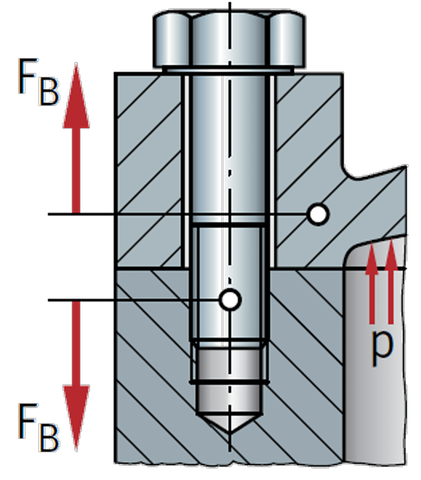
\includegraphics[width=0.48\linewidth,keepaspectratio]{graphics/v10_schraubenverbindung_einschraubverbindung.png}\hfill
    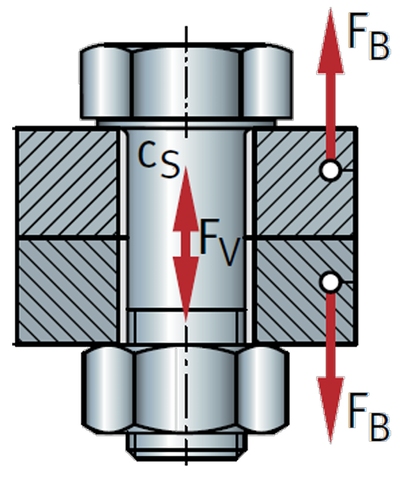
\includegraphics[width=0.48\linewidth,keepaspectratio]{graphics/v10_schraubenverbindung_durchsteckverbindung.png}%
  \end{minipage}%
  \hfill
  \begin{minipage}[c]{0.50\linewidth}%
    \raggedright
    \ZSFReadableOn
    \textbf{Gestaltungsfehler}:
    \begin{factlist}
    \item Kein Platz für Schraubenkopf
    \item Zu wenig Plattenmaterial
    \item Kein Spiel zwischen Schraubenkopf und Platten
    \item Unebene Auflagefläche für Schraubenkopf und -Mutter
    \end{factlist}
  \end{minipage}%
  \par
\end{figbox}
\ZSFindex{Einschraubverbindung}
\ZSFindex{Durchsteckverbindung}
\ZSFindex{Gestaltungsfehler}

\SubsectionBar[sec:schraubenbelastung]{Belastung der Schraube}
\ZSFindex{Anziehdrehmoment}

\begin{runintext}
Beim Anziehen entsteht ein zwei-achsiger Spannungszustand: \ZSFkeyword{Zugspannung} ($\ZSFscrewSigmaZ$) durch die Vorspannkraft $\ZSFscrewFv$ und \ZSFkeyword{Torsionsspannung} ($\ZSFscrewTauT$) durch Verdrehen gegen Gewindesteigung ($\ZSFscrewPhi$), Flanken- ($\ZSFscrewRhoPrime$) und Kopfreibung ($\ZSFscrewMuk$) beim Anziehdrehmoment $\ZSFscrewMA$.
\end{runintext}

\begin{formulabox}
\formulasources{Kräfte:~\ZSFsource{aus}{sec:verspannungsschaubild} \ $\cdot$ \ Gewindegrössen:~\ZSFsource{aus}{sec:gewinde} \ $\cdot$ \ $\ZSFscrewWtThree$:~\ZSFsource{bestimmen mit}{sec:widerstandsmoment}}
\ZSFkeyword*{Spannungen beim Anziehen}:~$\ZSFscrewSigmaZ = \frac{\ZSFscrewFsMax}{\ZSFscrewAs} \qquad \ZSFscrewTauT = \dfrac {\ZSFscrewMGMax}{\ZSFscrewWtThree}$

$\ZSFscrewMGMax = \tan(\ZSFscrewPhi + \ZSFscrewRhoPrime) \cdot \dfrac{\ZSFscrewFvMax \cdot \ZSFscrewDTwo}{2} \qquad \tan \ZSFscrewRhoPrime = \dfrac{\ZSFscrewMuG}{\cos(\ZSFscrewBeta/2)}$
\formulanote{$\ZSFscrewRhoPrime$:~Reibungswinkel \ $\cdot$ \ $\ZSFscrewFvMax$:~maximale Montagevorspannkraft (Axialkraft der Schraube) \ $\cdot$ \ $\ZSFscrewMG$:~Gewindemoment \ $\cdot$ \ $\ZSFscrewWtThree$:~Torsionswiderstandsmoment bei $\ZSFscrewDThree$}
\end{formulabox}

\begin{figbox}
\noindent
\begin{minipage}[c]{0.52\linewidth}
  \raggedright
  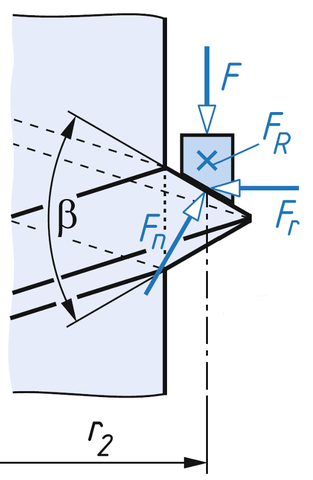
\includegraphics[width=0.48\linewidth,keepaspectratio]{graphics/v10_schraube_modell_spitzgewinde.png}\hfill
  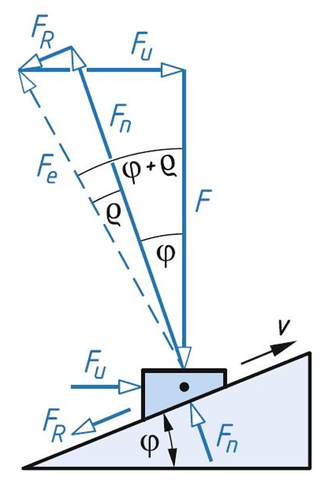
\includegraphics[width=0.48\linewidth,keepaspectratio]{graphics/v10_schraube_modell_reibung_steigung.png}
\end{minipage}\hfill
\begin{minipage}[c]{0.44\linewidth}
  \centering
  $\displaystyle \ZSFscrewFu = \ZSFscrewFv\cdot\tan(\ZSFscrewPhi + \ZSFscrewRhoPrime)$
  \par\ZSFgapS
  {\ZSFfontNote In der Grafik gilt: $\ZSFscrewF = \ZSFscrewFv$.\par}
\end{minipage}
\end{figbox}

\begin{formulabox}
\formulasources{Gewindegrössen:~\ZSFsource{aus}{sec:gewinde} \ $\cdot$ \ $\ZSFscrewFvMax$:~\ZSFsource{aus}{sec:verspannungsschaubild}}
\ZSFkeyword*{Modell: Reibung und Steigung}: $\ZSFscrewFu = \ZSFscrewF\cdot \tan(\ZSFscrewPhi + \ZSFscrewRho) \qquad \ZSFscrewMG = \dfrac{\ZSFscrewDTwo \cdot \ZSFscrewFu}{2} \qquad \ZSFscrewMu = \tan \ZSFscrewRho$

$\ZSFscrewFn = \dfrac{\ZSFscrewF}{cos(\ZSFscrewBeta/2)} \qquad \tan \ZSFscrewPhi = \dfrac{\ZSFscrewFu}{\ZSFscrewF}$
\formulanote{$\dots$ohne Reibung}
$\ZSFscrewFr = \ZSFscrewMu \cdot \ZSFscrewFn = \tan \ZSFscrewRho \cdot \ZSFscrewFn$
\formulanote{$\dots$mit Reibung}
\formulasep
\ZSFkeyword*{Anziehdrehmoment $\ZSFscrewMA$}: $\ZSFscrewMA = \ZSFscrewFvMax \cdot (\dfrac{\ZSFscrewDTwo}{2}\cdot \tan(\ZSFscrewPhi + \ZSFscrewRhoPrime) + \ZSFscrewMuk \cdot \dfrac{\ZSFscrewDk}{2}) \approx 0,17 \cdot \ZSFscrewFvMax \cdot \ZSFscrewD$
\formulanote{$\dots$Anziehdrehmoment mit Kopfreibung $\ZSFscrewMuk$ und maximaler Montagevorspannkraft $\ZSFscrewFvMax$. Bei Sechskant- und Zylinderschrauben, mit metrischem Gewinde ist $\ZSFscrewMuk = 0.12$ und $\dfrac{\ZSFscrewDk}{2} = 0.65\cdot \ZSFscrewD$.}
\end{formulabox}

\SubsectionBar[sec:verspannungsschaubild]{Verspannungsschaubild / Nachgiebigkeit}
\ZSFindex{Verspannungsschaubild}
\ZSFindex{Nachgiebigkeit}
\ZSFindex{Setzkraftverlust}

\begin{runintext}
Durch die \ZSFkeyword{Vorspannkraft} $\ZSFscrewFv$ der Schraube werden die Platten gestaucht ($\ZSFscrewFt$) und die Schrauben verlängert ($\ZSFscrewFs$), wobei $\ZSFscrewDeltaST$ die \ZSFkeyword*{Nachgiebigkeit} der Schraube/ verspannten Teile ist. Ebenfalls führt sie in den hochbelasteten Oberflächen zu plastischen Verformungen (\ZSFkeyword{Setzen}), also zur Abnahme der Vorspannkraft $\rightarrow$ \ZSFkeyword*{Setzkraftverlust} $\ZSFscrewFz$
\end{runintext}

\phantomsection\label{formula:screw-compliances}
\begin{formulabox}[Nachgiebigkeiten $\ZSFscrewDelta$]
\formulasources{Lage der $\ZSFscrewDeltai$:~\ZSFsource{aus}{sec:nachgiebigkeiten-orte}}
\[ \ZSFscrewF = \dfrac{\ZSFscrewFSmall}{\ZSFscrewDelta} \qquad \ZSFscrewDelta = \dfrac{\ZSFscrewL}{\ZSFscrewE\cdot \ZSFscrewA} \qquad \ZSFscrewR = \dfrac{\ZSFscrewE \cdot \ZSFscrewA}{\ZSFscrewL} \qquad \ZSFscrewFsT = \ZSFscrewDeltaST \cdot \ZSFscrewFv \]
\[ \ZSFscrewDeltaS = \ZSFscrewDeltaKo + \ZSFscrewDeltaOne + \ZSFscrewDeltaTwo + \ZSFscrewDeltaG + \ZSFscrewDeltaGe + \ZSFscrewDeltaM =\sum\ZSFscrewDeltai \]
\[ \ZSFscrewDeltaS = \frac{1}{\ZSFscrewES}\cdot\left(\frac{\ZSFscrewLKo}{\ZSFscrewAN}+\frac{\ZSFscrewLOne}{\ZSFscrewAdOne}+\frac{\ZSFscrewLTwo}{\ZSFscrewAdTwo}+\frac{\ZSFscrewLG}{\ZSFscrewAThree}+\frac{\ZSFscrewLGe}{\ZSFscrewAThree}\right)+\frac{\ZSFscrewLM}{\ZSFscrewEM\cdot \ZSFscrewAN} \]
\[ \ZSFscrewAN = \dfrac{\pi}{4}\cdot \ZSFscrewD^2 \qquad \ZSFscrewDeltaT = \dfrac{\ZSFscrewLk}{\ZSFscrewET \cdot \ZSFscrewAers} \]
\[ \ZSFscrewAers = \frac{\pi}{4}\cdot(\ZSFscrewDw^2 -\ZSFscrewDh^2) + \frac{\pi}{8}\cdot \ZSFscrewDw \cdot(\ZSFscrewDA - \ZSFscrewDw) \cdot ((\ZSFscrewX+1)^2-1) \]
\[ \ZSFscrewX = \sqrt[3]{\frac{\ZSFscrewLk\cdot \ZSFscrewDw}{\ZSFscrewDA^2}} \qquad \ZSFscrewDA \leq \ZSFscrewDw + \ZSFscrewLk \]
\end{formulabox}

\begin{figbox}[Nachgiebigkeit (Geometrie)]
\centering
\raisebox{\depth}{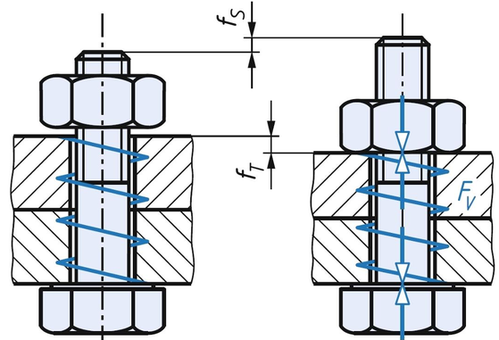
\includegraphics[width=0.33\linewidth,angle=-90,keepaspectratio]{graphics/v10_schraube_verspannungsschaubild.png}}%
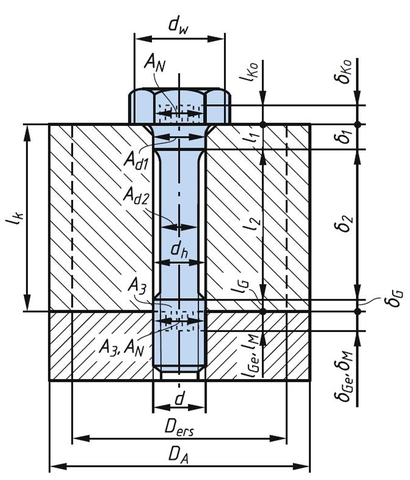
\includegraphics[width=0.36\linewidth,keepaspectratio]{graphics/v10_nachgiebigkeit_schraube.png}%
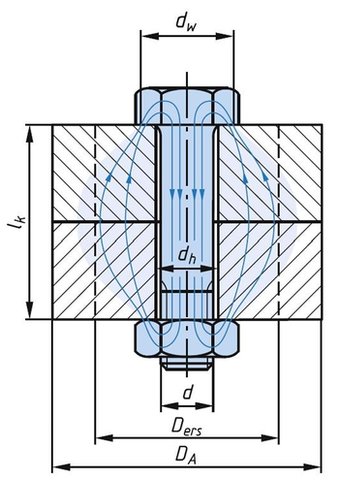
\includegraphics[width=0.30\linewidth,keepaspectratio]{graphics/v10_nachgiebigkeit_verspannte_teile.png}
\end{figbox}

\begin{formulabox}[Betriebs- und Vorspannkräfte]
\formulasources{$\ZSFscrewDeltaS$, $\ZSFscrewDeltaT$:~\ZSFsource{aus}{formula:screw-compliances} \ $\cdot$ \ $\ZSFscrewKA$:~\ZSFsource{aus}{sec:anziehwert}}
\[ \ZSFscrewFB = \ZSFscrewFBS + \ZSFscrewFBT \qquad \ZSFscrewFBS = \dfrac{\ZSFscrewDeltaT \cdot \ZSFscrewFB}{\ZSFscrewDeltaS + \ZSFscrewDeltaT} \qquad \ZSFscrewFBT = \dfrac{\ZSFscrewDeltaS \cdot \ZSFscrewFB}{\ZSFscrewDeltaS + \ZSFscrewDeltaT} \]
\[ \ZSFscrewFz = \dfrac{\ZSFscrewFSmallZ}{\ZSFscrewDeltaS + \ZSFscrewDeltaT} \qquad \ZSFscrewFsMax = \ZSFscrewFvMax + \ZSFscrewFBS \]
\[ \ZSFscrewFvMin = \ZSFscrewFkl + \ZSFscrewFz + \ZSFscrewFBT \qquad \ZSFscrewFvMax = \ZSFscrewKA \cdot \ZSFscrewFvMin \]
\formulanote{$\ZSFscrewFz =$ Setzkraftverlust, $\ZSFscrewFkl =$ Klemmkraft, $\ZSFscrewKA =$ Anziehfaktor, $\ZSFscrewFvMax =$ maximale Montagevorspannkraft, $\ZSFscrewFS =$ Schraubenkraft}
\end{formulabox}
\ZSFindex{Klemmkraft}
\ZSFindex{Montagevorspannkraft}

\begin{figbox}[Verspannungsschaubilder]
\centering
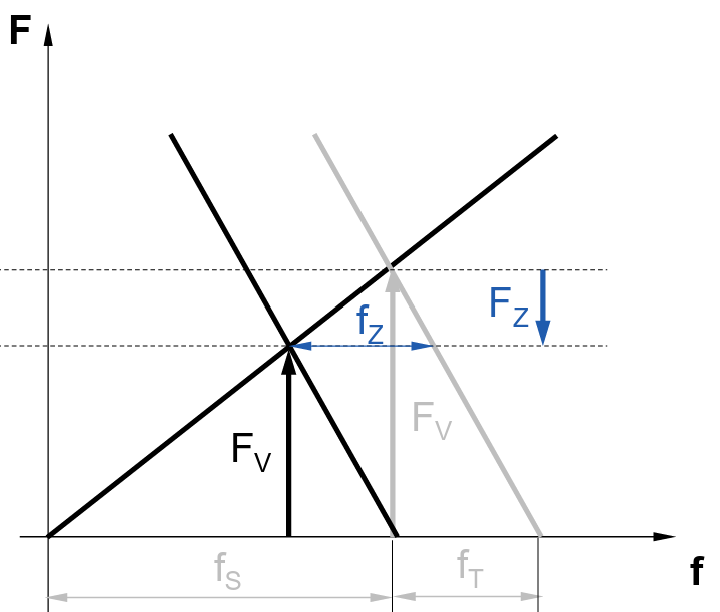
\includegraphics[width=0.22\linewidth,keepaspectratio]{graphics/v10_schraube_setzkraftverlust_diagramm.png}%
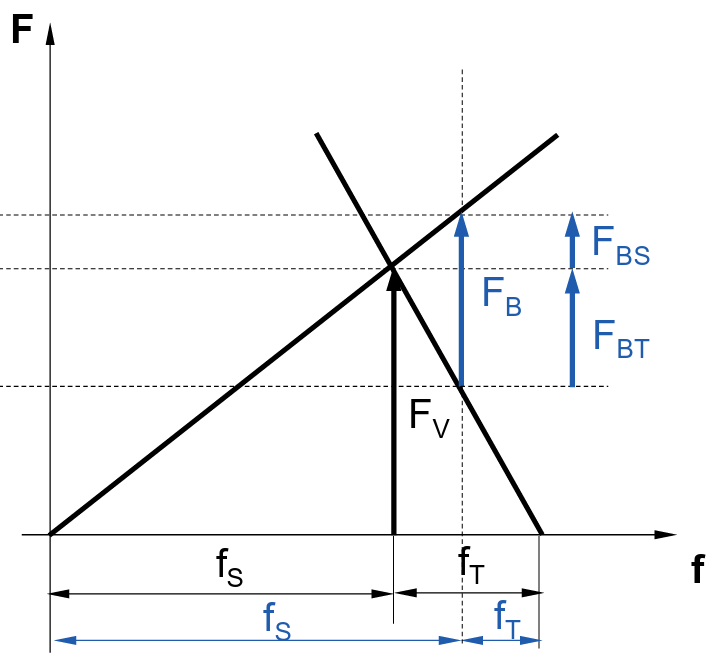
\includegraphics[width=0.22\linewidth,keepaspectratio]{graphics/v10_bolt_force_components_diagram.png}
\end{figbox}
